\linespread{1.5}
%use \usepackage{amsmath}
%use \usepackage{float}
\textbf{Solução}

\textbf{a)}
\begin{figure}[H]
    \centering
    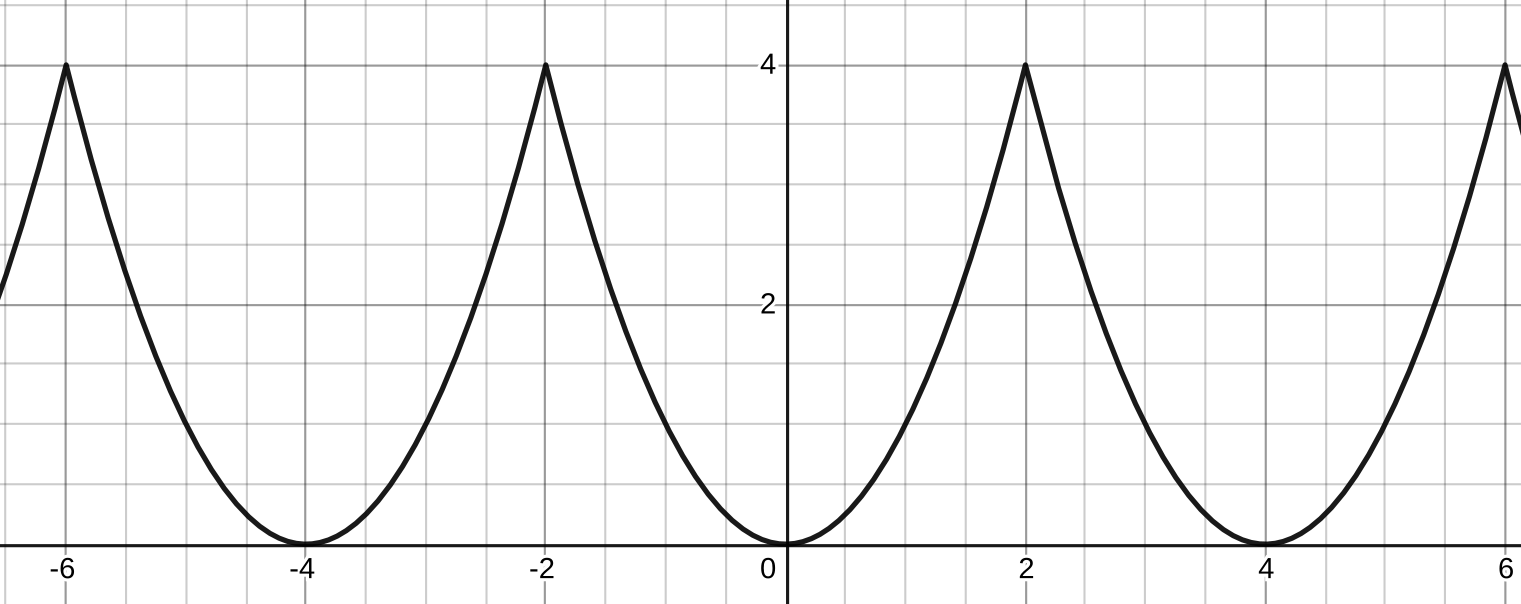
\includegraphics[width=0.6\linewidth]{fig/sf3a}
    \label{fig:sf3}
\end{figure}

\textbf{b)}
Dada a equação que define a série de Furier real:
\begin{equation}
    \label{eq:Fourierserie}
    f(t) = a_0 + \sum_{k=1}^\infty a_k\cos{(kwt)} + b_k\sin{(kwt)}
\end{equation}
Como a função $f(t) = t^2$ é uma função par, não se faz necessário calcular o coeficiente $b_k$, uma vez que ele acaba sendo igual a zero.
Quanto ao termo $a_k$, sabendo dos limites de integração temos que $T=4$ e este pode ser reescrito como:
\begin{equation*}
    a_k = \frac{2}{T}\int_{-T/2}^{T/2}t^2\cos{(kwt)}dt = \frac{1}{2}\int_{-2}^2t^2 \cos{(kwt)}dt
\end{equation*}
que pode ser resolvida por partes:
\begin{equation}
    \label{eq:sf3b}
    a_k = \frac{1}{2}\left\{\left[\frac{t^2\sin{(kwt)}}{kw}\right]^2_{-2} - \int_{-2}^2 \frac{2t\sin{(kwt)}}{kw}dt\right\} = \frac{1}{2}\left\{(I) - (II)\right\} 
\end{equation}
E novamente se faz necessário aplicar a integração por partes pra equação \textit{(II)}:
\begin{equation*}
    (II) = \int_{-2}^2 \frac{2t\sin{(kwt)}}{kw}dt = \left[\frac{-2t\cos{(kwt)}}{(kw)^2}\right]^2_{-2} - \int_{-2}^2 \frac{-2t\sin{(kwt)}}{(kw)^2}dt
\end{equation*}
\begin{equation*}
    = \left[\frac{-2t\cos{(kwt)}}{(kw)^2}\right]^2_{-2} - \left[\frac{-2\sin{(kwt)}}{(kw)^3}\right]^2_{-2} 
\end{equation*}
\begin{equation*}
    = \left[\left(\frac{-4\cos{(2kw)}}{(kw)^2}\right) - \left(\frac{4\cos{(-2kw)}}{(kw)^2}\right)\right] - \left[\left(\frac{-2\sin{(2kw)}}{(kw)^3}\right) - \left(\frac{-2\sin{(-2kw)}}{(kw)^3}\right)\right]
\end{equation*}
\begin{equation}
    \label{\eq:sf3bII}
    \boxed{(II) = \frac{-8\cos{(2kw)}}{(kw)^2} + \frac{4\sin{(2kw)}}{(kw)^3}}
\end{equation}
Resolvendo agora \textit{(I)}:
\begin{equation*}
    (I) = \left[\frac{t^2\sin{(kwt)}}{kw}\right]_{-2}^2 = \left(\frac{4\sin{(2kw)}}{kw}\right) - \left(\frac{4\sin{(-2kw)}}{kw}\right)
\end{equation*}
\begin{equation*}
    = \frac{4\sin{2kw}}{kw} + \frac{4\sin{(2kw)}}{kw}
\end{equation*}
\begin{equation}
    \label{eq:sf3bI}
    (I) = \frac{8\sin{(2kw)}}{kw}
\end{equation}
Substituído então \ref{eq:sf3bI} e \ref{\eq:sf3bII} em \ref{eq:sf3b}, obtemos:
\begin{equation*}
    a_k = \frac{1}{2}\left\{\frac{8\sin{(2kw)}}{kw} + \frac{8\cos{(2kw)}}{(kw)^2} - \frac{4\sin{(2kw)}}{(kw)^3}\right\}
\end{equation*}
Sabendo que $T = 4$ e portanto que $w = \frac{2\pi}{4} = \frac{\pi}{2}$. Logo:
\begin{equation*}
    a_k = \frac{1}{2}\left\{\frac{16\sin{(k\pi)}}{k\pi} +  \frac{32\cos{(k\pi)}}{(k\pi)^2} - \frac{32\sin{(k\pi)}}{(k\pi)^3}\right\}
\end{equation*}
\begin{equation*}
    \frac{8\sin{(k\pi)}}{k\pi} +  \frac{16\cos{(k\pi)}}{(k\pi)^2} - \frac{16\sin{(k\pi)}}{(k\pi)^3}
\end{equation*}

Se sabe também que para $k\in\N$ e $k\geq1$, $\sin{k\pi} = 0$ e $\cos{k\pi} = (-1)^k$. Assim:
\begin{equation}
    \label{eq:sf3ak}
    a_k = \frac{16}{(k\pi)^2}(-1)^k
\end{equation}

Agora o coeficiente $a_0$ é dado por:
\begin{equation}
    \label{eq:sf3a0}
    a_0 = \frac{1}{4}\int_{-2}^2 t^2dt = \frac{1}{4}\left[\frac{t^3}{3}\right]_{-2}^2 = \frac{1}{4}\left[\frac{8}{3} + \frac{8}{3}\right] = 4/3
\end{equation}

Substituindo então \ref{eq:sf3a0}, \ref{eq:sf3ak} e $b_k = 0$ em \ref{eq:Fourierserie}, temos que a série de Fourier de $f(t) = t^2$ é dada por:
\begin{equation*}
    \boxed{f(t) = \frac{4}{3} + \sum_{k=1}^\infty \frac{16}{(k\pi)^2}(-1)^k\cos{\left(\frac{k\pit}{2}\right)}}
\end{equation*}